%\documentclass[10pt]{beamer}
%\usetheme{amcg}

%\begin{document}

\section{Shear Instability}
\subsection{Get the files}

\frame{
  \frametitle{Get the example files}
Download the files:

{\tt \quad cd /data/<username> 

\quad bzr co --lightweight  $\mathtt{\backslash}$

\qquad lp:$\mathtt{\sim}$j-percival/fluidity/shear-examples
}

Set some examples running:

{\tt \quad cd shear-examples

\quad fluidity travelling\_wave\_periodised.flml\&\\
\quad fluidity shear\_low\_res\_periodised.flml\&\\
\quad fluidity shear\_high\_res\_periodised.flml\&\\
}
}

\frame{
  \frametitle{Get the example files}
Open up the slides for reference:

Feel free to skip ahead.

{\tt \quad bzr update}\\
{\tt \quad xdg-open slides.pdf\&}\\
}




\subsection{Setting up periodicity in fluidity}


\frame[Periodicity in Fluidity]{
To set up a periodic problem in fluidity there are two steps which must be performed:
\begin{enumerate}
  \item Create an initial mesh file so that boundaries which are to become periodic are compatible.
  \item Write a {\tt .flml} file which tells fluidity which boundaries are periodic and how to get from one side to another.
\end{enumerate}
}

\frame{
\frametitle{Periodicity in Fluidity - GMSH}
GMSH provides a set of commands

{\tt \quad Periodic Line \{{\it line ids}\} = \{$\pm${\it line ids}\};\\}
{\tt \quad Periodic Surface {\it surf. id} \{$\pm${\it line ids}\} = {\it surf. id} \{$\pm${\it line ids}\};\\}

Tells gmsh to mesh one line/surface identically to another. Note orientation matters! Unfortantly not available from GUI.

\vskip 0.5cm

Open {\tt periodic\_example.geo} in the {\tt periodic\_example} directory in a text editor to see an example of use. Mesh it as before.\\
{\tt\quad cd periodic\_example}\\
{\tt\quad  gmsh -2 periodic\_example.geo}\\
}

\frame{
\frametitle{Periodicity in Fluidity - Diamond}

Now to tell fluidity to make a periodic topological mesh. Open a related options file in diamond:\\
{\tt \quad diamond periodic\_example.flml\&}\\
Look under the geometry settings. New mesh has been added with periodic boundary conditions applied to it.
}




\frame{
  \frametitle{Periodicity in Fluidity - Running}
  \begin{itemize}
    \item The serial fixed mesh problem can then be run directly.\\
      {\tt \quad fluidity periodic\_example.flml\&}
    \item To use adaptivity, or run in parallel must use {\tt periodise} tool to create full periodic connectivity information.\\
    \item Lets run the command and look as the periodic topology:\\
      {\tt \quad periodise periodic\_example.flml\&}
      {\tt \quad gmsh periodic\_example\_periodic.msh}
    \item Note: cannot curently run parallel+periodic+adaptive [in development]
  \end{itemize}
}

\frame{
  \frametitle{Periodicity in Fluidity - Running}
  \begin{itemize}
    \item Some things to note:
      \begin{itemize}
        \item Can't run full set parallel computation +periodic bcs + mesh adaptivity yet, (coming soon).
        \item Sometimes issues with periodic+Galerkin projection for adaptivity; Consistent interpolation is safe.
        \item With adaptivity output mesh may (will) not span exact region of initial mesh, but will always be close.
      \end{itemize}
  \end{itemize}
}

\frame{
  \frametitle{Shear Instability}
  \begin{itemize}
    \item Examples simulating  two dimensional hydrodynamic instability:\\
      \begin{enumerate}
        \item Dispersion behind an approximate travelling wave.\\
        \item Growth of Kelvin-Helmholtz billows in a shear layer.
      \end{enumerate}
    \item Evolution of the shear flow is modelled in a  stratified, incompressible fluid is modelled in a 100m deep domain with horizontal period 20 m.\\
  \end{itemize}
}

\frame{
  \frametitle{Travelling wave example - Simulation setup: Initial conditions}
  Example
  \begin{itemize}
    \item Takes analytic solution of travelling wave solution from a two layer model (Choi-Camassa equations).
    \item Run these data forward with full Boussinesq equations.
    \item Adjustment creates dispersive tail left behind the wave, similar to results seen in lab.
    \item No normal flow boundary conditions on the bottom and top.\\
    \item Periodic boundary conditions on sides.\\
  \end{itemize}
}

\frame{
  \frametitle{Shear Instability example - Initial conditions}
  Example
  \begin{itemize}
    \item $u=0.38\tanh(z-10)$, $v=0$\\
    \item $\rho=1000-T$ $T=tanh(5z)-1/10\cos(\pi*x/20)/cosh(x/100.0)$\\
    \item No normal flow boundary conditions on the bottom and top.\\
    \item Periodic boundary conditions on sides \\
  \end{itemize}
}

\frame{
  \frametitle{Shear Instability - Simulation setup: Initial conditions}
  Example
  \begin{itemize}
    \item $u=(0.38\tanh(z-10),0)$\\
    \item $\rho=1000-T$ $T=tanh(5z)-1/10\cos(\pi*x/20)/cosh(x/100.0)$\\
    \item No normal flow boundary conditions on the bottom and top.\\
    \item Periodic boundary conditions on sides \\
  \end{itemize}
}

\frame{
  \frametitle{Shear Instability - Numerical results Low Res}
\begin{figure}[H]
{
        \centering
 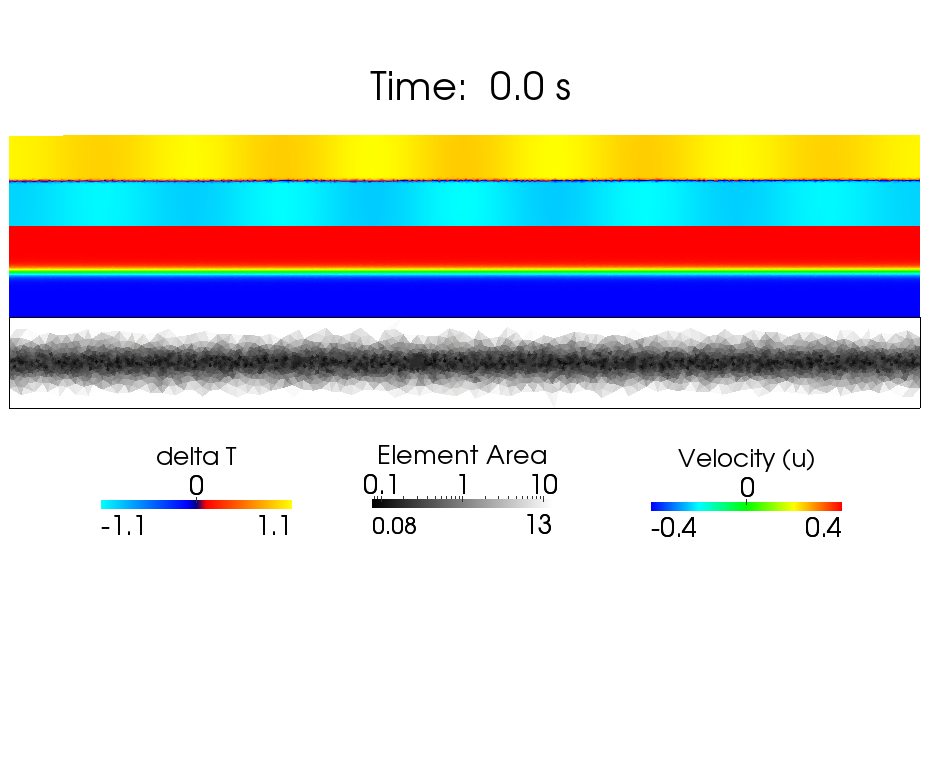
\includegraphics[width=\columnwidth]{./shear_instability/Low_res_result_0.png}
}
\end{figure}
}

\frame{
  \frametitle{Shear Instability - Numerical results Low Res}
\begin{figure}[H]
{
        \centering
 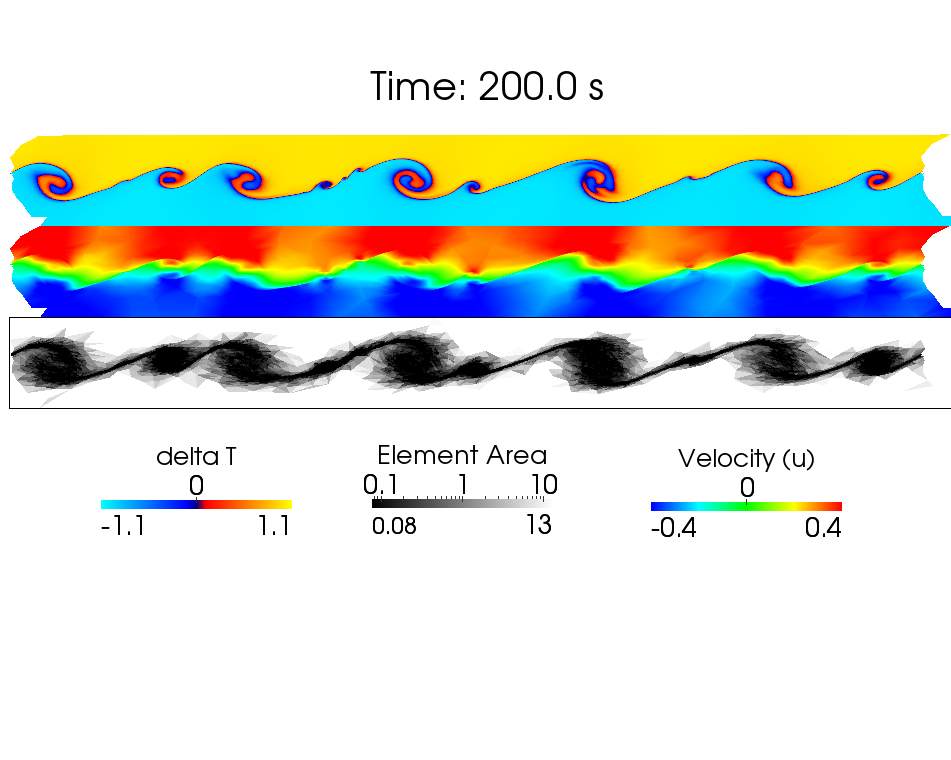
\includegraphics[width=\columnwidth]{./shear_instability/Low_res_result_200.png}
}
\end{figure}
}

\frame{
  \frametitle{Shear Instability - Numerical results Low Res}
\begin{figure}[H]
{
        \centering
 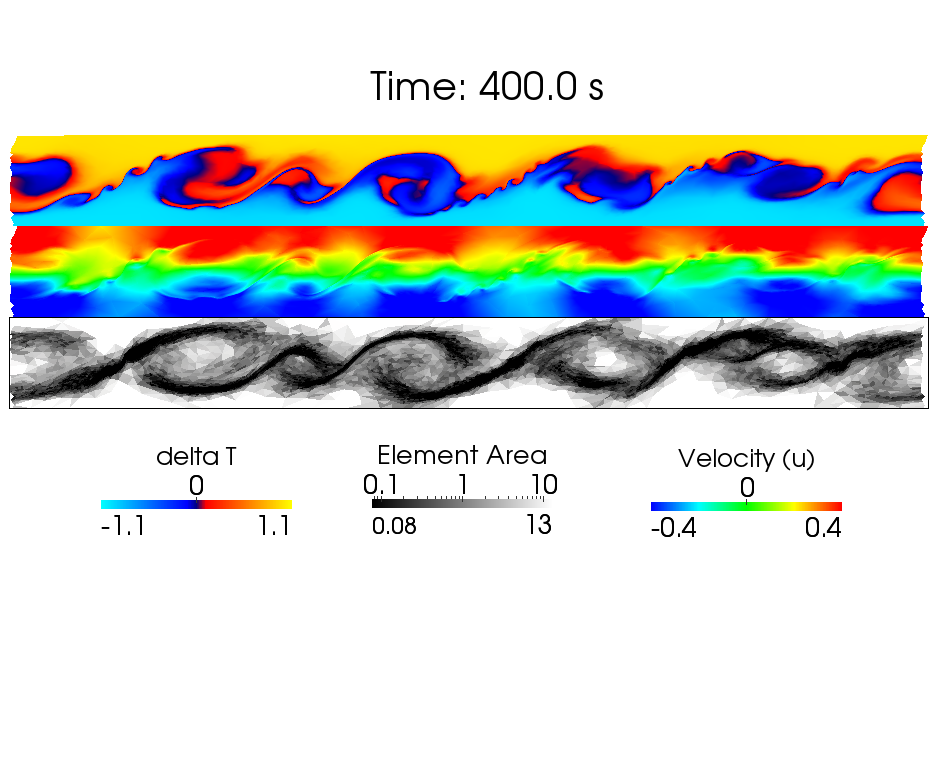
\includegraphics[width=\columnwidth]{./shear_instability/Low_res_result_400.png}
}
\end{figure}
}


\frame{
  \frametitle{Shear Instability - Numerical results - High Res}
\begin{figure}[H]
{
        \centering
 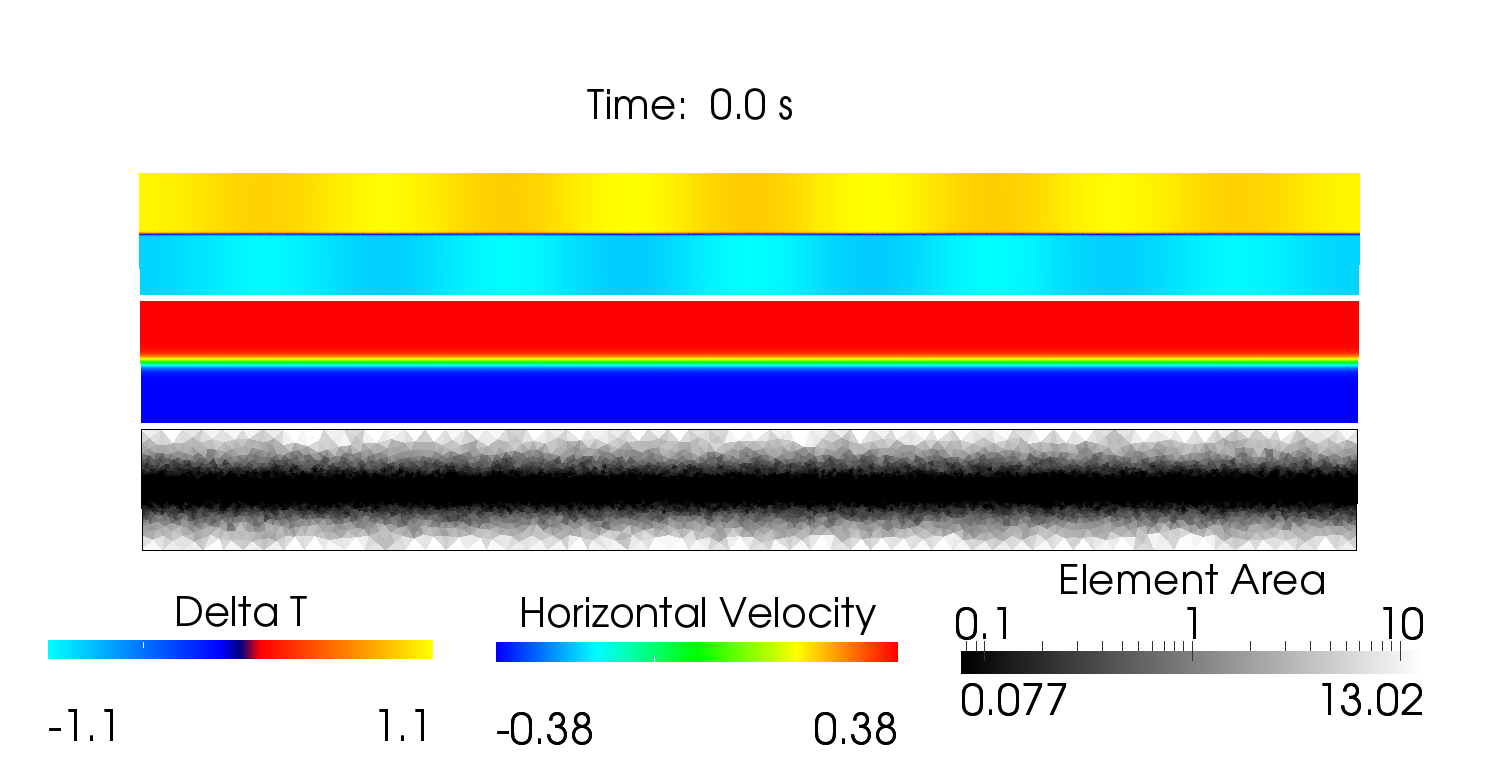
\includegraphics[width=\columnwidth]{./shear_instability/High_res_result_0.png}
}
\end{figure}
}

\frame{
  \frametitle{Shear Instability - Numerical results}
\begin{figure}[H]
{
        \centering
 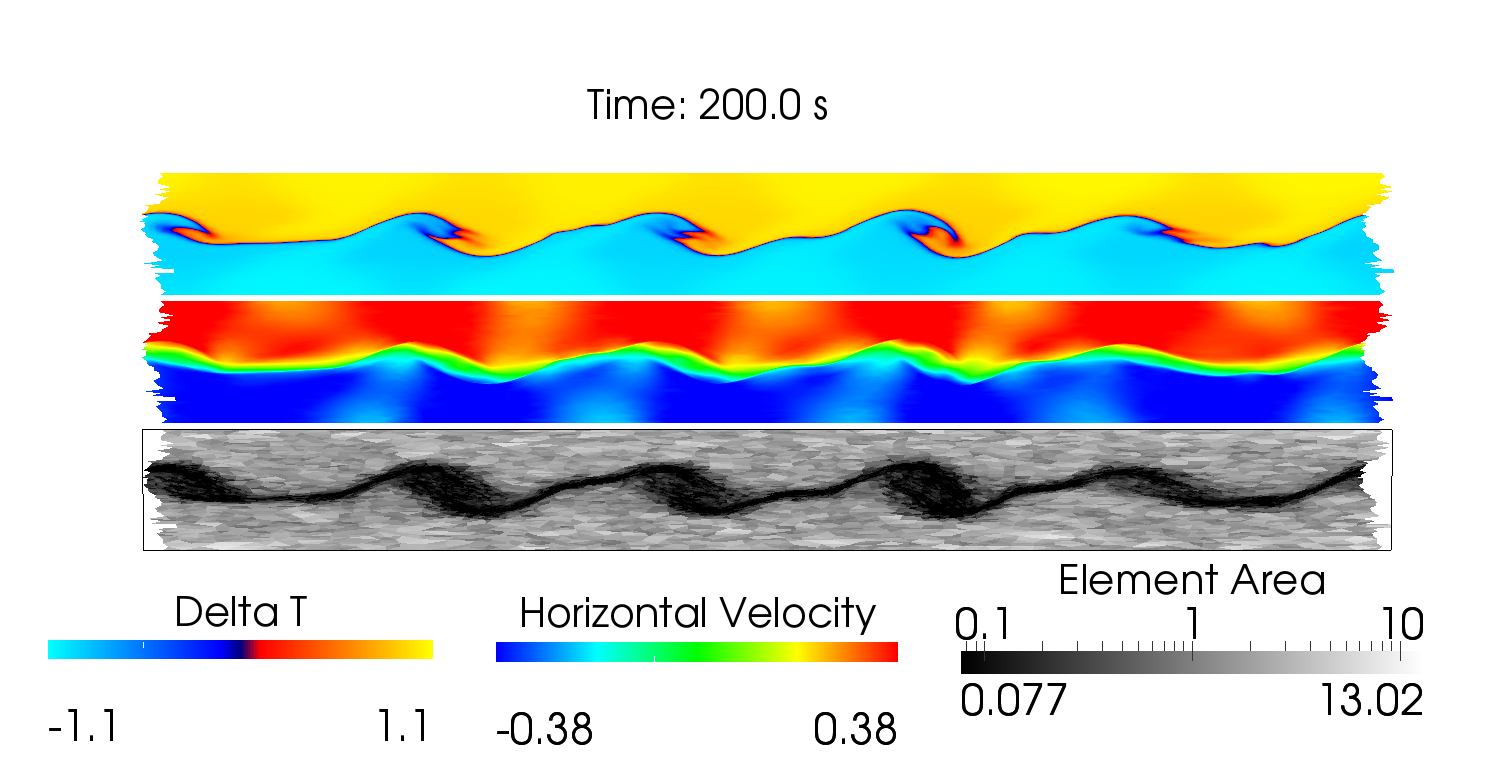
\includegraphics[width=\columnwidth]{./shear_instability/High_res_result_200.png}
}
\end{figure}
}

\frame{
  \frametitle{Shear Instability - Numerical results - High Res}
\begin{figure}[H]
{
        \centering
 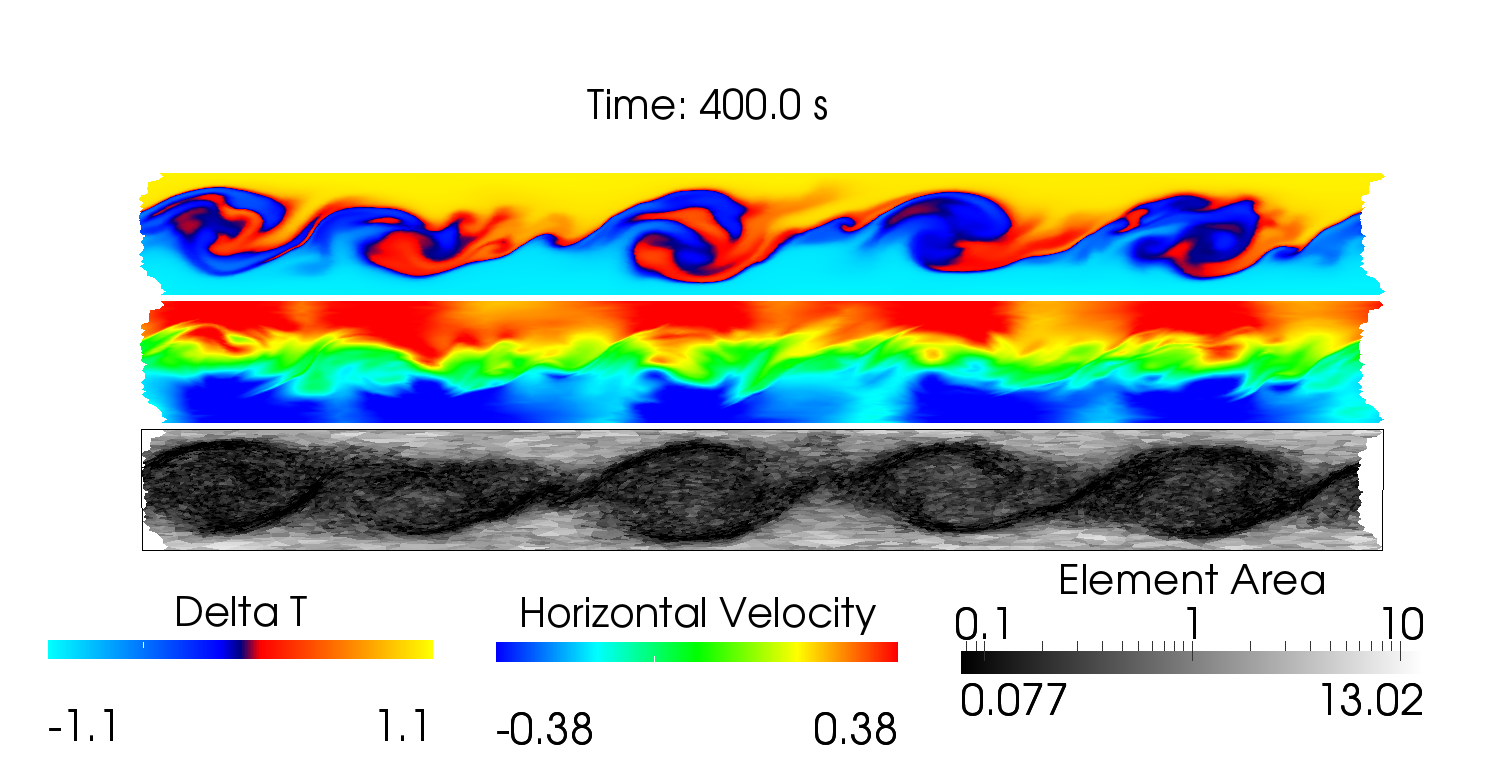
\includegraphics[width=\columnwidth]{./shear_instability/High_res_result_400.png}
}
\end{figure}
}





\frame{
  \frametitle{Shear Instability - Exercises}
 \begin{itemize}
 \item Add adaptivity based on velocity.\\
 \item Disable the adaptivity option to run on a fixed mesh.\\
 \item Alter the temperature perturbation.\\
 \item Alter the intensity of the shear flow.
 \end{itemize}
}

%\end{document}
